\section{eo\-Binary\-Hypervolume\-Indicator$<$ EOFitness $>$ Class Template Reference}
\label{classeoBinaryHypervolumeIndicator}\index{eoBinaryHypervolumeIndicator@{eoBinaryHypervolumeIndicator}}
Functor Binary hypervolume indicator for {\bf eo\-Pareto\-Fitness}.  


{\tt \#include $<$eo\-Binary\-Quality\-Indicator.h$>$}

Inheritance diagram for eo\-Binary\-Hypervolume\-Indicator$<$ EOFitness $>$::\begin{figure}[H]
\begin{center}
\leavevmode
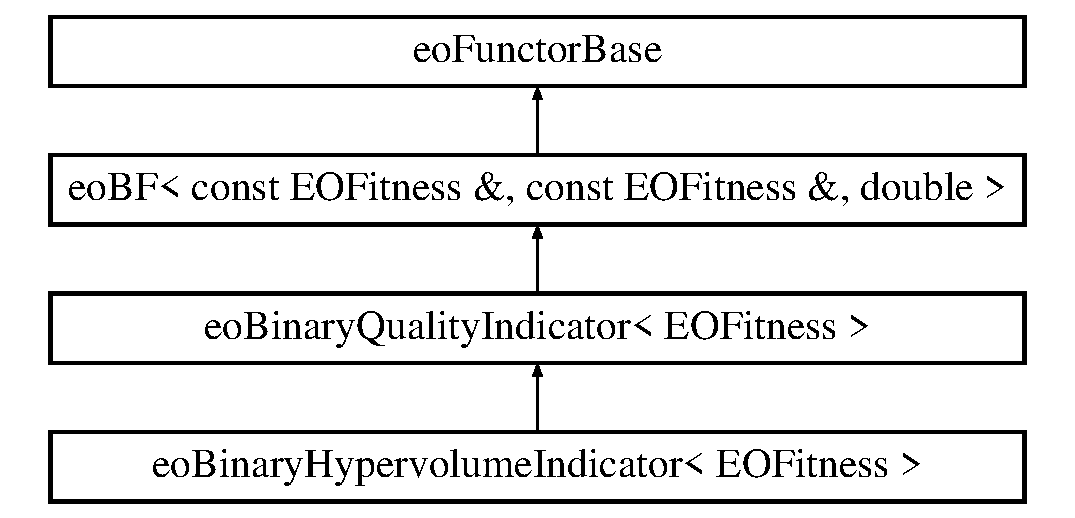
\includegraphics[height=4cm]{classeoBinaryHypervolumeIndicator}
\end{center}
\end{figure}
\subsection*{Public Member Functions}
\begin{CompactItemize}
\item 
{\bf eo\-Binary\-Hypervolume\-Indicator} (double \_\-rho)
\begin{CompactList}\small\item\em constructor \item\end{CompactList}\item 
double {\bf operator()} (const EOFitness \&\_\-fitness\_\-eo1, const EOFitness \&\_\-fitness\_\-eo2)
\begin{CompactList}\small\item\em indicator value of the hypervolume of the portion of the objective space that is dominated by individual \_\-eo1 but not by individual \_\-eo2 (don't forget to set the bounds before the call of this function) \item\end{CompactList}\end{CompactItemize}
\subsection*{Private Types}
\begin{CompactItemize}
\item 
typedef EOFitness::fitness\_\-traits {\bf traits}\label{classeoBinaryHypervolumeIndicator_abde225206c55671bd585cc41cbfab1c}

\begin{CompactList}\small\item\em fitness traits \item\end{CompactList}\end{CompactItemize}
\subsection*{Private Member Functions}
\begin{CompactItemize}
\item 
double {\bf hypervolume\-Indicator\-Value} (const EOFitness \&\_\-fitness\_\-eo1, const EOFitness \&\_\-fitness\_\-eo2, const unsigned \_\-i\-Obj, const bool \_\-flag=false)
\begin{CompactList}\small\item\em computation of the hypervolume of the portion of the objective space that is dominated by individual \_\-eo1 but not by individual \_\-eo2 \item\end{CompactList}\item 
double {\bf hypervolume\-Indicator\-Value\-Min} (const EOFitness \&\_\-fitness\_\-eo1, const EOFitness \&\_\-fitness\_\-eo2, const unsigned \_\-i\-Obj, const bool \_\-flag)
\begin{CompactList}\small\item\em computation of the hypervolume of the portion of the objective space that is dominated by individual \_\-eo1 but not by individual \_\-eo2 in case of a minimization on the objective \_\-i\-Obj \item\end{CompactList}\item 
double {\bf hypervolume\-Indicator\-Value\-Max} (const EOFitness \&\_\-fitness\_\-eo1, const EOFitness \&\_\-fitness\_\-eo2, const unsigned \_\-i\-Obj, const bool \_\-flag)
\begin{CompactList}\small\item\em computation of the hypervolume of the portion of the objective space that is dominated by individual \_\-eo1 but not by individual \_\-eo2 in case of a maximization on the objective \_\-i\-Obj \item\end{CompactList}\end{CompactItemize}
\subsection*{Private Attributes}
\begin{CompactItemize}
\item 
double {\bf rho}\label{classeoBinaryHypervolumeIndicator_02fdfd1b2aa8071cdd3d395777d709a5}

\begin{CompactList}\small\item\em reference point for the hypervolume calculation \item\end{CompactList}\end{CompactItemize}


\subsection{Detailed Description}
\subsubsection*{template$<$class EOFitness$>$ class eo\-Binary\-Hypervolume\-Indicator$<$ EOFitness $>$}

Functor Binary hypervolume indicator for {\bf eo\-Pareto\-Fitness}. 



Definition at line 217 of file eo\-Binary\-Quality\-Indicator.h.

\subsection{Constructor \& Destructor Documentation}
\index{eoBinaryHypervolumeIndicator@{eo\-Binary\-Hypervolume\-Indicator}!eoBinaryHypervolumeIndicator@{eoBinaryHypervolumeIndicator}}
\index{eoBinaryHypervolumeIndicator@{eoBinaryHypervolumeIndicator}!eoBinaryHypervolumeIndicator@{eo\-Binary\-Hypervolume\-Indicator}}
\subsubsection{\setlength{\rightskip}{0pt plus 5cm}template$<$class EOFitness$>$ {\bf eo\-Binary\-Hypervolume\-Indicator}$<$ EOFitness $>$::{\bf eo\-Binary\-Hypervolume\-Indicator} (double {\em \_\-rho})\hspace{0.3cm}{\tt  [inline]}}\label{classeoBinaryHypervolumeIndicator_8b1dedf93c1936ea7efa9b19913d8773}


constructor 

\begin{Desc}
\item[Parameters:]
\begin{description}
\item[{\em double}]\_\-rho reference point for the hypervolume calculation (rho must not be smaller than 1) \end{description}
\end{Desc}


Definition at line 227 of file eo\-Binary\-Quality\-Indicator.h.

References eo\-Binary\-Hypervolume\-Indicator$<$ EOFitness $>$::rho.

\subsection{Member Function Documentation}
\index{eoBinaryHypervolumeIndicator@{eo\-Binary\-Hypervolume\-Indicator}!operator()@{operator()}}
\index{operator()@{operator()}!eoBinaryHypervolumeIndicator@{eo\-Binary\-Hypervolume\-Indicator}}
\subsubsection{\setlength{\rightskip}{0pt plus 5cm}template$<$class EOFitness$>$ double {\bf eo\-Binary\-Hypervolume\-Indicator}$<$ EOFitness $>$::operator() (const EOFitness \& {\em \_\-fitness\_\-eo1}, const EOFitness \& {\em \_\-fitness\_\-eo2})\hspace{0.3cm}{\tt  [inline, virtual]}}\label{classeoBinaryHypervolumeIndicator_d418f42f086a3221c60ad9149b5df9d0}


indicator value of the hypervolume of the portion of the objective space that is dominated by individual \_\-eo1 but not by individual \_\-eo2 (don't forget to set the bounds before the call of this function) 

\begin{Desc}
\item[Parameters:]
\begin{description}
\item[{\em EOFitness}]\& \_\-fitness\_\-eo1 the fitness of the first individual \item[{\em EOFitness}]\& \_\-fitness\_\-eo2 the fitness of the second individual \end{description}
\end{Desc}


Implements {\bf eo\-BF$<$ const EOFitness \&, const EOFitness \&, double $>$}.

Definition at line 250 of file eo\-Binary\-Quality\-Indicator.h.

References eo\-Binary\-Hypervolume\-Indicator$<$ EOFitness $>$::hypervolume\-Indicator\-Value().\index{eoBinaryHypervolumeIndicator@{eo\-Binary\-Hypervolume\-Indicator}!hypervolumeIndicatorValue@{hypervolumeIndicatorValue}}
\index{hypervolumeIndicatorValue@{hypervolumeIndicatorValue}!eoBinaryHypervolumeIndicator@{eo\-Binary\-Hypervolume\-Indicator}}
\subsubsection{\setlength{\rightskip}{0pt plus 5cm}template$<$class EOFitness$>$ double {\bf eo\-Binary\-Hypervolume\-Indicator}$<$ EOFitness $>$::hypervolume\-Indicator\-Value (const EOFitness \& {\em \_\-fitness\_\-eo1}, const EOFitness \& {\em \_\-fitness\_\-eo2}, const unsigned {\em \_\-i\-Obj}, const bool {\em \_\-flag} = {\tt false})\hspace{0.3cm}{\tt  [inline, private]}}\label{classeoBinaryHypervolumeIndicator_9c12e672eaf7ed2b17cab9b96af911e6}


computation of the hypervolume of the portion of the objective space that is dominated by individual \_\-eo1 but not by individual \_\-eo2 

\begin{Desc}
\item[Parameters:]
\begin{description}
\item[{\em EOFitness}]\& \_\-fitness\_\-eo1 the fitness of the first individual \item[{\em EOFitness}]\& \_\-fitness\_\-eo2 the fitness of the second individual \item[{\em unsigned}]\_\-i\-Obj number of objectives (used for iteration) \item[{\em bool}]\_\-flag = false (only used for iteration) \end{description}
\end{Desc}


Definition at line 285 of file eo\-Binary\-Quality\-Indicator.h.

References eo\-Binary\-Quality\-Indicator$<$ EOFitness $>$::bounds, eo\-Binary\-Hypervolume\-Indicator$<$ EOFitness $>$::hypervolume\-Indicator\-Value\-Max(), and eo\-Binary\-Hypervolume\-Indicator$<$ EOFitness $>$::hypervolume\-Indicator\-Value\-Min().

Referenced by eo\-Binary\-Hypervolume\-Indicator$<$ EOFitness $>$::hypervolume\-Indicator\-Value\-Max(), eo\-Binary\-Hypervolume\-Indicator$<$ EOFitness $>$::hypervolume\-Indicator\-Value\-Min(), and eo\-Binary\-Hypervolume\-Indicator$<$ EOFitness $>$::operator()().\index{eoBinaryHypervolumeIndicator@{eo\-Binary\-Hypervolume\-Indicator}!hypervolumeIndicatorValueMin@{hypervolumeIndicatorValueMin}}
\index{hypervolumeIndicatorValueMin@{hypervolumeIndicatorValueMin}!eoBinaryHypervolumeIndicator@{eo\-Binary\-Hypervolume\-Indicator}}
\subsubsection{\setlength{\rightskip}{0pt plus 5cm}template$<$class EOFitness$>$ double {\bf eo\-Binary\-Hypervolume\-Indicator}$<$ EOFitness $>$::hypervolume\-Indicator\-Value\-Min (const EOFitness \& {\em \_\-fitness\_\-eo1}, const EOFitness \& {\em \_\-fitness\_\-eo2}, const unsigned {\em \_\-i\-Obj}, const bool {\em \_\-flag})\hspace{0.3cm}{\tt  [inline, private]}}\label{classeoBinaryHypervolumeIndicator_6c9b9a5279ad7894b4563e205f13e98b}


computation of the hypervolume of the portion of the objective space that is dominated by individual \_\-eo1 but not by individual \_\-eo2 in case of a minimization on the objective \_\-i\-Obj 

\begin{Desc}
\item[Parameters:]
\begin{description}
\item[{\em EOFitness}]\& \_\-fitness\_\-eo1 the fitness of the first individual \item[{\em EOFitness}]\& \_\-fitness\_\-eo2 the fitness of the second individual \item[{\em unsigned}]\_\-i\-Obj index of the objective \item[{\em bool}]\_\-flag (only used for iteration) \end{description}
\end{Desc}


Definition at line 320 of file eo\-Binary\-Quality\-Indicator.h.

References eo\-Binary\-Quality\-Indicator$<$ EOFitness $>$::bounds, eo\-Binary\-Hypervolume\-Indicator$<$ EOFitness $>$::hypervolume\-Indicator\-Value(), and eo\-Binary\-Hypervolume\-Indicator$<$ EOFitness $>$::rho.

Referenced by eo\-Binary\-Hypervolume\-Indicator$<$ EOFitness $>$::hypervolume\-Indicator\-Value().\index{eoBinaryHypervolumeIndicator@{eo\-Binary\-Hypervolume\-Indicator}!hypervolumeIndicatorValueMax@{hypervolumeIndicatorValueMax}}
\index{hypervolumeIndicatorValueMax@{hypervolumeIndicatorValueMax}!eoBinaryHypervolumeIndicator@{eo\-Binary\-Hypervolume\-Indicator}}
\subsubsection{\setlength{\rightskip}{0pt plus 5cm}template$<$class EOFitness$>$ double {\bf eo\-Binary\-Hypervolume\-Indicator}$<$ EOFitness $>$::hypervolume\-Indicator\-Value\-Max (const EOFitness \& {\em \_\-fitness\_\-eo1}, const EOFitness \& {\em \_\-fitness\_\-eo2}, const unsigned {\em \_\-i\-Obj}, const bool {\em \_\-flag})\hspace{0.3cm}{\tt  [inline, private]}}\label{classeoBinaryHypervolumeIndicator_df2903822dbcd0a906dabf4cb6e05bfb}


computation of the hypervolume of the portion of the objective space that is dominated by individual \_\-eo1 but not by individual \_\-eo2 in case of a maximization on the objective \_\-i\-Obj 

\begin{Desc}
\item[Parameters:]
\begin{description}
\item[{\em EOFitness}]\& \_\-fitness\_\-eo1 the fitness of the first individual \item[{\em EOFitness}]\& \_\-fitness\_\-eo2 the fitness of the second individual \item[{\em unsigned}]\_\-i\-Obj index of the objective \item[{\em bool}]\_\-flag (only used for iteration) \end{description}
\end{Desc}


Definition at line 374 of file eo\-Binary\-Quality\-Indicator.h.

References eo\-Binary\-Quality\-Indicator$<$ EOFitness $>$::bounds, eo\-Binary\-Hypervolume\-Indicator$<$ EOFitness $>$::hypervolume\-Indicator\-Value(), and eo\-Binary\-Hypervolume\-Indicator$<$ EOFitness $>$::rho.

Referenced by eo\-Binary\-Hypervolume\-Indicator$<$ EOFitness $>$::hypervolume\-Indicator\-Value().

The documentation for this class was generated from the following file:\begin{CompactItemize}
\item 
eo\-Binary\-Quality\-Indicator.h\end{CompactItemize}
